% Options for packages loaded elsewhere
\PassOptionsToPackage{unicode}{hyperref}
\PassOptionsToPackage{hyphens}{url}
\PassOptionsToPackage{dvipsnames,svgnames,x11names}{xcolor}
%
\documentclass[
  10pt,
  ignorenonframetext,
]{beamer}
\usepackage{pgfpages}
\setbeamertemplate{caption}[numbered]
\setbeamertemplate{caption label separator}{: }
\setbeamercolor{caption name}{fg=normal text.fg}
\beamertemplatenavigationsymbolsempty
% Prevent slide breaks in the middle of a paragraph
\widowpenalties 1 10000
\raggedbottom
\setbeamertemplate{part page}{
  \centering
  \begin{beamercolorbox}[sep=16pt,center]{part title}
    \usebeamerfont{part title}\insertpart\par
  \end{beamercolorbox}
}
\setbeamertemplate{section page}{
  \centering
  \begin{beamercolorbox}[sep=12pt,center]{part title}
    \usebeamerfont{section title}\insertsection\par
  \end{beamercolorbox}
}
\setbeamertemplate{subsection page}{
  \centering
  \begin{beamercolorbox}[sep=8pt,center]{part title}
    \usebeamerfont{subsection title}\insertsubsection\par
  \end{beamercolorbox}
}
\AtBeginPart{
  \frame{\partpage}
}
\AtBeginSection{
  \ifbibliography
  \else
    \frame{\sectionpage}
  \fi
}
\AtBeginSubsection{
  \frame{\subsectionpage}
}
\usepackage{amsmath,amssymb}
\usepackage{lmodern}
\usepackage{setspace}
\usepackage{iftex}
\ifPDFTeX
  \usepackage[T1]{fontenc}
  \usepackage[utf8]{inputenc}
  \usepackage{textcomp} % provide euro and other symbols
\else % if luatex or xetex
  \usepackage{unicode-math}
  \defaultfontfeatures{Scale=MatchLowercase}
  \defaultfontfeatures[\rmfamily]{Ligatures=TeX,Scale=1}
\fi
% Use upquote if available, for straight quotes in verbatim environments
\IfFileExists{upquote.sty}{\usepackage{upquote}}{}
\IfFileExists{microtype.sty}{% use microtype if available
  \usepackage[]{microtype}
  \UseMicrotypeSet[protrusion]{basicmath} % disable protrusion for tt fonts
}{}
\makeatletter
\@ifundefined{KOMAClassName}{% if non-KOMA class
  \IfFileExists{parskip.sty}{%
    \usepackage{parskip}
  }{% else
    \setlength{\parindent}{0pt}
    \setlength{\parskip}{6pt plus 2pt minus 1pt}}
}{% if KOMA class
  \KOMAoptions{parskip=half}}
\makeatother
\usepackage{xcolor}
\geometry{left = 1cm, right = 0.5cm, top = 0.5cm, bottom = 0.5cm}
\newif\ifbibliography
\usepackage{color}
\usepackage{fancyvrb}
\newcommand{\VerbBar}{|}
\newcommand{\VERB}{\Verb[commandchars=\\\{\}]}
\DefineVerbatimEnvironment{Highlighting}{Verbatim}{commandchars=\\\{\}}
% Add ',fontsize=\small' for more characters per line
\usepackage{framed}
\definecolor{shadecolor}{RGB}{248,248,248}
\newenvironment{Shaded}{\begin{snugshade}}{\end{snugshade}}
\newcommand{\AlertTok}[1]{\textcolor[rgb]{0.94,0.16,0.16}{#1}}
\newcommand{\AnnotationTok}[1]{\textcolor[rgb]{0.56,0.35,0.01}{\textbf{\textit{#1}}}}
\newcommand{\AttributeTok}[1]{\textcolor[rgb]{0.77,0.63,0.00}{#1}}
\newcommand{\BaseNTok}[1]{\textcolor[rgb]{0.00,0.00,0.81}{#1}}
\newcommand{\BuiltInTok}[1]{#1}
\newcommand{\CharTok}[1]{\textcolor[rgb]{0.31,0.60,0.02}{#1}}
\newcommand{\CommentTok}[1]{\textcolor[rgb]{0.56,0.35,0.01}{\textit{#1}}}
\newcommand{\CommentVarTok}[1]{\textcolor[rgb]{0.56,0.35,0.01}{\textbf{\textit{#1}}}}
\newcommand{\ConstantTok}[1]{\textcolor[rgb]{0.00,0.00,0.00}{#1}}
\newcommand{\ControlFlowTok}[1]{\textcolor[rgb]{0.13,0.29,0.53}{\textbf{#1}}}
\newcommand{\DataTypeTok}[1]{\textcolor[rgb]{0.13,0.29,0.53}{#1}}
\newcommand{\DecValTok}[1]{\textcolor[rgb]{0.00,0.00,0.81}{#1}}
\newcommand{\DocumentationTok}[1]{\textcolor[rgb]{0.56,0.35,0.01}{\textbf{\textit{#1}}}}
\newcommand{\ErrorTok}[1]{\textcolor[rgb]{0.64,0.00,0.00}{\textbf{#1}}}
\newcommand{\ExtensionTok}[1]{#1}
\newcommand{\FloatTok}[1]{\textcolor[rgb]{0.00,0.00,0.81}{#1}}
\newcommand{\FunctionTok}[1]{\textcolor[rgb]{0.00,0.00,0.00}{#1}}
\newcommand{\ImportTok}[1]{#1}
\newcommand{\InformationTok}[1]{\textcolor[rgb]{0.56,0.35,0.01}{\textbf{\textit{#1}}}}
\newcommand{\KeywordTok}[1]{\textcolor[rgb]{0.13,0.29,0.53}{\textbf{#1}}}
\newcommand{\NormalTok}[1]{#1}
\newcommand{\OperatorTok}[1]{\textcolor[rgb]{0.81,0.36,0.00}{\textbf{#1}}}
\newcommand{\OtherTok}[1]{\textcolor[rgb]{0.56,0.35,0.01}{#1}}
\newcommand{\PreprocessorTok}[1]{\textcolor[rgb]{0.56,0.35,0.01}{\textit{#1}}}
\newcommand{\RegionMarkerTok}[1]{#1}
\newcommand{\SpecialCharTok}[1]{\textcolor[rgb]{0.00,0.00,0.00}{#1}}
\newcommand{\SpecialStringTok}[1]{\textcolor[rgb]{0.31,0.60,0.02}{#1}}
\newcommand{\StringTok}[1]{\textcolor[rgb]{0.31,0.60,0.02}{#1}}
\newcommand{\VariableTok}[1]{\textcolor[rgb]{0.00,0.00,0.00}{#1}}
\newcommand{\VerbatimStringTok}[1]{\textcolor[rgb]{0.31,0.60,0.02}{#1}}
\newcommand{\WarningTok}[1]{\textcolor[rgb]{0.56,0.35,0.01}{\textbf{\textit{#1}}}}
\setlength{\emergencystretch}{3em} % prevent overfull lines
\providecommand{\tightlist}{%
  \setlength{\itemsep}{0pt}\setlength{\parskip}{0pt}}
\setcounter{secnumdepth}{-\maxdimen} % remove section numbering
\usepackage{float}
\usepackage{booktabs}
\usepackage{array}
\usepackage{multirow}
\setbeamertemplate{itemize item}{$\diamond$}
\setbeamertemplate{itemize subitem}{\scriptsize$\diamond$}
\setbeamertemplate{navigation symbols}{}
\setbeamertemplate{footline}[page number]
\definecolor{blue}{RGB}{0,114,178}
\definecolor{red}{RGB}{213,94,0}
\definecolor{yellow}{RGB}{240,228,66}
\definecolor{green}{RGB}{0,158,115}
\ifLuaTeX
  \usepackage{selnolig}  % disable illegal ligatures
\fi
\IfFileExists{bookmark.sty}{\usepackage{bookmark}}{\usepackage{hyperref}}
\IfFileExists{xurl.sty}{\usepackage{xurl}}{} % add URL line breaks if available
\urlstyle{same} % disable monospaced font for URLs
\hypersetup{
  pdftitle={Econometrics: Multiple Regression and Applications},
  pdfauthor={Duong Trinh},
  colorlinks=true,
  linkcolor={blue},
  filecolor={Maroon},
  citecolor={Blue},
  urlcolor={Blue},
  pdfcreator={LaTeX via pandoc}}

\title{Econometrics: Multiple Regression and Applications}
\subtitle{ECON4004: LAB 1}
\author{Duong Trinh}
\date{February 7, 2024}
\institute{University of Glasgow}

\begin{document}
\frame{\titlepage}

\setstretch{1.5}
\begin{frame}{Intro}
\protect\hypertarget{intro}{}
\begin{itemize}
\tightlist
\item
  Duong Trinh

  \begin{itemize}
  \tightlist
  \item
    PhD Student in Economics (Bayesian Microeconometrics)
  \item
    Email: \underline{Duong.Trinh@glasgow.ac.uk}
  \end{itemize}
\end{itemize}

\vspace{3mm}

\begin{itemize}
\tightlist
\item
  ECON4004-LB01

  \begin{itemize}
  \tightlist
  \item
    Wednesday 10am -12 pm
  \item
    5 sessions (7-Feb, 14-Feb, 21-Feb, 28-Feb, 6-March)
  \item
    ST ANDREWS:357
  \end{itemize}
\item
  ECON4004-LB02

  \begin{itemize}
  \tightlist
  \item
    Wednesday 12-2 pm
  \item
    5 sessions (7-Feb, 14-Feb, 21-Feb, 28-Feb, 6-March)
  \item
    ST ANDREWS:357
  \end{itemize}
\end{itemize}
\end{frame}

\begin{frame}{Record Attendance}
\protect\hypertarget{record-attendance}{}
\end{frame}

\begin{frame}[fragile]{Picture the Scenario}
\protect\hypertarget{picture-the-scenario}{}
\begin{itemize}
\tightlist
\item
  \textbf{Objective:} Investigate the effect of fertility on women labor
  supply behaviour (\emph{with a focus on Instrumental Variable
  approach}).
\end{itemize}

\vspace{0.8mm}

\begin{itemize}
\tightlist
\item
  \textbf{Dataset:} \texttt{fertility.dta}

  \begin{itemize}
  \tightlist
  \item
    from 1980 U.S. Census.
  \item
    contains information on \(254,654\) married women aged 21--35 with
    two or more children.
  \end{itemize}
\end{itemize}

\vspace{0.8mm}

\begin{itemize}
\tightlist
\item
  \textbf{Key variables:}

  \begin{itemize}
  \tightlist
  \item
    \texttt{weeksm1}: weeks worked (labor supply)
  \item
    \texttt{morekids}: the indicator variable denoting having more than
    2 children (fertility)
  \item
    \texttt{samesex}: equals to \(1\) if the first two children are of
    the same sex (boy--boy or girl--girl) and equal to \(0\) otherwise.
  \end{itemize}
\end{itemize}
\end{frame}

\begin{frame}[fragile]{Questions (S\&W Exercise E12.1)}
\protect\hypertarget{LGQ}{}
\begin{block}{Linear regression}
\protect\hypertarget{linear-regression}{}
\footnotesize \protect\hyperlink{LGCG}{(\textgreater\textgreater review)}
\normalsize

\begin{enumerate}
[(a)]
\item
  Regress \texttt{weeksm1} on \texttt{morekids} using OLS. On average,
  do women with more than two children work less than women with two
  children? How much less?
\item
  Explain why the OLS regression estimated in (a) is inappropriate for
  estimating the causal effect of fertility (\texttt{morekids}) on labor
  supply (\texttt{weeksm1}).
\end{enumerate}
\end{block}
\end{frame}

\begin{frame}[fragile]{Questions (S\&W Exercise E12.1)}
\protect\hypertarget{IVQ}{}
\begin{block}{IV regression with a single regressor and a single
instrument}
\protect\hypertarget{iv-regression-with-a-single-regressor-and-a-single-instrument}{}
\footnotesize\protect\hyperlink{IVCG}{(\textgreater\textgreater review)}
\normalsize

\begin{enumerate}
[(a)]
\setcounter{enumi}{2}
\item
  Are couples whose first two children are of the same sex more likely
  to have a third child? Is the effect large? Is it statistically
  significant?
\item
  Explain why \texttt{samesex} is a valid instrument for the IV
  regression of weeks worked on \texttt{morekids}.
\item
  Is \texttt{samesex} a weak instrument?
\item
  Estimate the IV regression of weeks worked on \texttt{morekids}, using
  \texttt{samesex} as an instrument. How large is the fertility effect
  on labor supply? How can we test whether \texttt{morekids} is
  endogenous?
\end{enumerate}
\end{block}
\end{frame}

\begin{frame}[fragile]{Questions (S\&W Exercise E12.1)}
\protect\hypertarget{IVCQ}{}
\begin{block}{IV regression with additional control variables}
\protect\hypertarget{iv-regression-with-additional-control-variables}{}
\footnotesize\protect\hyperlink{IVCCG}{(\textgreater\textgreater review)}
\normalsize

\begin{enumerate}
[(a)]
\setcounter{enumi}{6}
\tightlist
\item
  Include the variables \texttt{agem1}, \texttt{black}, \texttt{hispan},
  and \texttt{othrace} in the labor supply regression (treating these
  variables as exogenous).
\end{enumerate}

\begin{itemize}
\item
  Do the results change? Explain why or why not.
\item
  Does the instrumental variable remain relevant? Why?
\item
  Does the test of endogeneity give different results than in (f)? What
  can we conclude about the endogeneity of \texttt{morekids}?
\end{itemize}
\end{block}
\end{frame}

\begin{frame}{(a) Regress \texttt{weeksm1} on \texttt{morekids} using
OLS.}
\protect\hypertarget{q1-regOLS}{}
\begin{itemize}
\item
  Linear regression model \[
  \color{red}{weeksm1_i = \beta_0 + \beta_1 \cdot morekids_i + u_i}
  \]
\item
  OLS estimation results
  \footnotesize \protect\hyperlink{res1-regOLS}{(\textgreater\textgreater stata)}
  \normalsize \[
  \underset{(se)}{\widehat{weeksm1}} = \underset{(0.0561)}{21.0684} -  \underset{(0.0871)}{5.3867} \cdot morekids \qquad R^2=0.0143
  \]
\item
  The slope estimate \(\hat{\beta}_1^{OLS} \approx -5.39\) indicates
  that women with more than two children work \(5.39\) fewer weeks per
  year than women with two or fewer children \emph{on average}.
\end{itemize}
\end{frame}

\begin{frame}{(b) Explain why this result is inappropriate for
estimating ~the causal effect of fertility on labor supply.}
\protect\hypertarget{LRissue}{}
\begin{itemize}
\tightlist
\item
  Both fertility and labor supply are choice variables which are
  endogenously determined. Women's age, education, wage, partner's
  income, or unobservable characteristics related to tastes for children
  and working might affect both desired fertility and employment
  decisions simultaneously.
\end{itemize}

\vspace{3mm}

\begin{itemize}
\tightlist
\item
  Ignoring these factors and using the simple linear regression only may
  distort (overestimate or underestimate) the true causal effect.
  \footnotesize \protect\hyperlink{OVB}{(\textgreater\textgreater review)}
  \normalsize
\end{itemize}
\end{frame}

\begin{frame}[fragile]{(c) Are couples whose first two children are of
the same sex more likely to have a third child?}
\protect\hypertarget{q2-regFirstStage}{}
\begin{itemize}
\item
  Linear regression model \[
  \color{green}{morekids_i = \delta_0 + \delta_1 \cdot samesex_i + v_i}
  \]
\item
  Estimation results
  \footnotesize \protect\hyperlink{res2-regFirstStage}{(\textgreater\textgreater stata)}
  \normalsize \[
  \underset{(se)}{\widehat{morekids}} = \underset{(0.0013)}{0.3464} + \underset{(0.0019)}{0.0675} \cdot samesex \qquad R^2=0.0048
  \]
\item
  \(\hat{\delta}_1 \approx 0.0675\) suggests that couples with
  \texttt{samesex} = 1 are \(6.75\%\) more likely to have an additional
  child than couples with \texttt{samesex} = 0 \emph{on average}.
\item
  The effect is highly significant (\(\text{t-statistic} = 35.2\)).
\end{itemize}
\end{frame}

\begin{frame}[fragile]{(d) Explain why \texttt{samesex} is a valid
instrument for the IV regression of \texttt{weeksm1} on
\texttt{morekids}.}
\protect\hypertarget{d-explain-why-samesex-is-a-valid-instrument-for-the-iv-regression-of-weeksm1-on-morekids.}{}
\[
\color{red}{weeksm1_i = \beta_0 + \beta_1 \cdot morekids_i + u_i}
\]

\begin{itemize}
\tightlist
\item
  Two conditions for a valid instrument:

  \begin{enumerate}
  \tightlist
  \item
    \emph{Relevant}? \(\text{corr}(samesex_i,morekids_i) \neq 0\)?\\
    Plausibly: The effect of \texttt{samesex} on \texttt{morekids} is
    statistically significant, as discussed in (c). The first stage
    \(F-statistic = 1238.17\) is large. \vspace{2mm}
  \item
    \emph{Exogenous}? \(\text{corr}(samesex_i,u_i) = 0\)?\\
    Plausibly: \texttt{samesex} is random and is unrelated to any of the
    other variables in the model including the error term in the labor
    supply equation.
  \end{enumerate}

  \vspace{2mm}

  \(\Rightarrow\) Together, these imply that \texttt{samesex} is a valid
  instrument.
\end{itemize}
\end{frame}

\begin{frame}[fragile]{(e) Is \texttt{samesex} a weak instrument?}
\protect\hypertarget{e-is-samesex-a-weak-instrument}{}
\begin{itemize}
\item
  This is related to the first condition - \emph{Instrument Relevance}
  in (d).
\item
  First-stage regression \[
  \color{green}{morekids_i = \delta_0 + \delta_1 \cdot samesex_i + v_i}
  \]
\item
  The instrument is \emph{weak} if \(\delta_1\) is either zero or nearly
  zero, i.e.~it explains very little of the variation in
  \texttt{morekids}. From (c), this is not the case of \texttt{samesex}.
  \footnotesize \protect\hyperlink{res2-regFirstStage}{(\textgreater\textgreater stata)}
  \normalsize
\end{itemize}
\end{frame}

\begin{frame}[fragile]{(f) Estimate the IV regression of
\texttt{weeksm1} on \texttt{morekids}, using \texttt{samesex} as an
instrument.}
\protect\hypertarget{f-estimate-the-iv-regression-of-weeksm1-on-morekids-using-samesex-as-an-instrument.}{}
TSLS has two stages - two regressions:

\begin{enumerate}
\item
  Regress \(morekids_i\) on \(samesex_i\) to isolate the part of
  \texttt{morekids} that is uncorrelated with \(u\) \[
  \color{green}{morekids_i = \delta_0 + \delta_1 \cdot samesex_i + v_i}
  \] Then, compute the predicted values
  \(\widehat{morekids}_i = \hat\delta_0 + \hat\delta_1 \cdot samesex_i\)
  for \(i = 1,\ldots,n.\)
\item
  Regress \(weeksm1_i\) on \(\widehat{morekids}_i\) \[
  \color{red}{weeksm1_i = \beta_0 + \beta_1 \cdot \widehat{morekids}_i + u_i}
  \] We eventually obtain \(\hat{\beta}_1^{TSLS}\), which is the TSLS
  estimator.
\end{enumerate}
\end{frame}

\begin{frame}[fragile]{{[}SN{]} Stata command for IV regression of \(Y\)
on a single endogenous \(X\) instrumented by \(Z\)}
\protect\hypertarget{sn-stata-command-for-iv-regression-of-y-on-a-single-endogenous-x-instrumented-by-z}{}
OLS standard errors from the second stage regression are not correct as
they do not take into account the estimation in the first stage when
\(\hat{X}\) is estimated. \textcolor{blue}{\texttt{ivregress}} command
in Stata adjusts for this 2 stage process.

\small

\begin{Shaded}
\begin{Highlighting}[]
\NormalTok{* ivregress 2sls yvar (xvar = IV), }\FunctionTok{r}
\CommentTok{// report result of intrinsic interest with 2SLS estimate}
\end{Highlighting}
\end{Shaded}

\begin{Shaded}
\begin{Highlighting}[]
\NormalTok{* ivregress 2sls yvar (xvar = IV), }\FunctionTok{r}\NormalTok{ first}
\CommentTok{// report additional result from first{-}stage regression}
\end{Highlighting}
\end{Shaded}

\begin{Shaded}
\begin{Highlighting}[]
\NormalTok{* ivregress 2sls yvar (xvar = IV), }\FunctionTok{r}
\NormalTok{* }\KeywordTok{estat}\NormalTok{ firststage}
\CommentTok{// report first{-}stage regression statistics}
\end{Highlighting}
\end{Shaded}

\begin{Shaded}
\begin{Highlighting}[]
\NormalTok{* ivregress 2sls yvar (xvar = IV), }\FunctionTok{r}
\NormalTok{* }\KeywordTok{estat}\NormalTok{ endog}
\CommentTok{// perform tests of the endogeneity of xvar}
\end{Highlighting}
\end{Shaded}
\end{frame}

\begin{frame}[fragile]{{[}SN{]} IV regression with \(Y:weeksm1\),
\(X:morekids\), and intrument \(Z:samesex\)}
\protect\hypertarget{sn-iv-regression-with-yweeksm1-xmorekids-and-intrument-zsamesex}{}
\small

\begin{Shaded}
\begin{Highlighting}[]
\NormalTok{* ivregress 2sls yvar (xvar = IV), }\FunctionTok{r}
\end{Highlighting}
\end{Shaded}

\begin{center}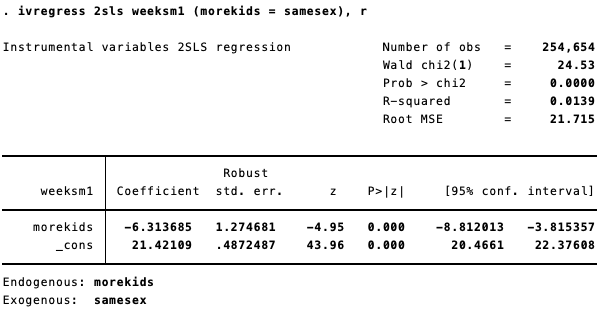
\includegraphics[width=1\linewidth]{pictures/res3-ivregress} \end{center}
\end{frame}

\begin{frame}[fragile]{{[}SN{]} Another way to check Instrument
Relevance}
\protect\hypertarget{IVestatFirstStage}{}
\small

\begin{Shaded}
\begin{Highlighting}[]
\NormalTok{* ivregress 2sls yvar (xvar = IV), }\FunctionTok{r}
\NormalTok{* }\KeywordTok{estat}\NormalTok{ firststage}
\end{Highlighting}
\end{Shaded}

\begin{center}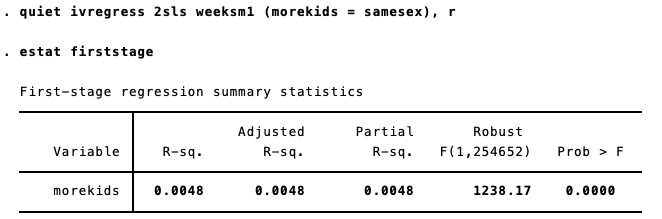
\includegraphics[width=1\linewidth]{pictures/res4-estatFirstStage} \end{center}

\(\Rightarrow\) The instrument \texttt{samesex} remains relevant!

\footnotesize \protect\hyperlink{res2-regFirstStage}{(\textgreater\textgreater compare)}
\normalsize
\end{frame}

\begin{frame}{(f) How large is the fertility effect on labor supply?}
\protect\hypertarget{f-how-large-is-the-fertility-effect-on-labor-supply}{}
\begin{itemize}
\item
  Estimation result \[
  \hat{\beta}_1^{TSLS} \approx -6.31, \quad \text{robust s.e} \approx 1.27 
  \] suggests that that women with more than two children work \(6.31\)
  fewer weeks per year than women with two or fewer children \emph{on
  average}. \vspace{1mm}
\item
  Homogeneous effects: If the causal effect is the same for every
  individual, the result above has \emph{causal interpretation}.
  \vspace{1mm}
\item
  Heterogeneous effects: \emph{we will discuss later}.
\end{itemize}
\end{frame}

\begin{frame}[fragile]{(f) Test endogeneity of regressor \(X:morekids\)}
\protect\hypertarget{f-test-endogeneity-of-regressor-xmorekids}{}
\begin{Shaded}
\begin{Highlighting}[]
\NormalTok{* ivregress 2sls yvar (xvar = IV), }\FunctionTok{r}
\NormalTok{* }\KeywordTok{estat}\NormalTok{ endog}
\end{Highlighting}
\end{Shaded}

\begin{center}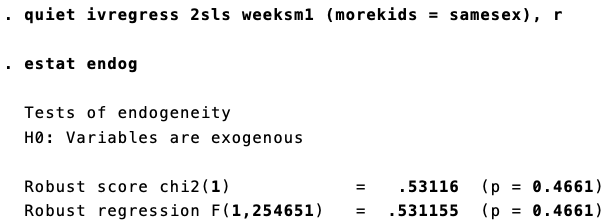
\includegraphics[width=0.7\linewidth]{pictures/res5-estatEndog} \end{center}

\(\Rightarrow\) Result of robustified DWH test suggests variable
\texttt{morekids} is unlikely to be endogenous, as the \(p-values\) are
well above \(0.1\).
\end{frame}

\begin{frame}{(g) Include (exogenous) variables \texttt{agem1},
\texttt{black}, \texttt{hispan}, and \texttt{othrace} in the labor
supply regression.}
\protect\hypertarget{g-include-exogenous-variables-agem1-black-hispan-and-othrace-in-the-labor-supply-regression.}{}
\begin{enumerate}
\item
  Regress \(morekids_i\) on \(samesex_i\) and all exogenous variables
  \begin{equation*}
  \begin{split}
  \color{green}{morekids_i} &\color{green}{= \delta_0 + \delta_1 \cdot samesex_i + \delta_2 \cdot agem1_i + \delta_3 \cdot black_i + }\\
  &\hspace{24pt} \color{green}{+ \delta_4 \cdot hispan_i + \delta_5 \cdot othrace_i + v_i}
  \end{split}
  \end{equation*} Then, compute the predicted values
  \(\widehat{morekids}_i\) for \(i = 1,\ldots,n.\)
\item
  Regress \(weeksm1_i\) on \(\widehat{morekids}_i\) \begin{equation*}
  \begin{split}
  \color{red}{weeksm1_i} &\color{red}{= \beta_0 + \beta_1 \cdot \widehat{morekids}_i + \beta_2 \cdot agem1_i + \beta_3 \cdot black_i + } \\ 
  &\hspace{24pt} \color{red}{+\beta_4 \cdot hispan_i + \beta_5 \cdot othrace_i + u_i}
  \end{split}
  \end{equation*} We eventually obtain \(\hat{\beta}_1^{TSLS}\), which
  is the TSLS estimator.
\end{enumerate}
\end{frame}

\begin{frame}[fragile]{{[}SN{]} Stata command for IV regression of \(Y\)
on a single endogenous \(X\) instrumented by \(Z\), and several
exogenous \(W\)s}
\protect\hypertarget{sn-stata-command-for-iv-regression-of-y-on-a-single-endogenous-x-instrumented-by-z-and-several-exogenous-ws}{}
Implement \textcolor{blue}{\texttt{ivregress}} command with additional
exogenous variables

\small

\begin{Shaded}
\begin{Highlighting}[]
\NormalTok{* ivregress 2sls yvar wvar1 wvar2 wvark (xvar = IV), }\FunctionTok{r}
\CommentTok{// report result of intrinsic interest with 2SLS estimate}
\end{Highlighting}
\end{Shaded}

\begin{Shaded}
\begin{Highlighting}[]
\NormalTok{* ivregress 2sls yvar wvar1 wvar2 wvark (xvar = IV), }\FunctionTok{r}\NormalTok{ first}
\CommentTok{// report additional result from first{-}stage regression}
\end{Highlighting}
\end{Shaded}

\begin{Shaded}
\begin{Highlighting}[]
\NormalTok{* ivregress 2sls yvar wvar1 wvar2 wvark (xvar = IV), }\FunctionTok{r}
\NormalTok{* }\KeywordTok{estat}\NormalTok{ firststage}
\CommentTok{// report first{-}stage regression statistics}
\end{Highlighting}
\end{Shaded}

\begin{Shaded}
\begin{Highlighting}[]
\NormalTok{* ivregress 2sls yvar wvar1 wvar2 wvark (xvar = IV), }\FunctionTok{r}
\NormalTok{* }\KeywordTok{estat}\NormalTok{ endog}
\CommentTok{// perform tests of the endogeneity of xvar}
\end{Highlighting}
\end{Shaded}
\end{frame}

\begin{frame}[fragile]{(g) IV regression with \(Y:weeksm1\),
\(X:morekids\), \(Z:samesex\), and additional exogenous regressors}
\protect\hypertarget{g-iv-regression-with-yweeksm1-xmorekids-zsamesex-and-additional-exogenous-regressors}{}
\small

\begin{Shaded}
\begin{Highlighting}[]
\NormalTok{* ivregress 2sls yvar wvar1 wvar2 wvark (xvar = IV), }\FunctionTok{r}
\end{Highlighting}
\end{Shaded}

\begin{center}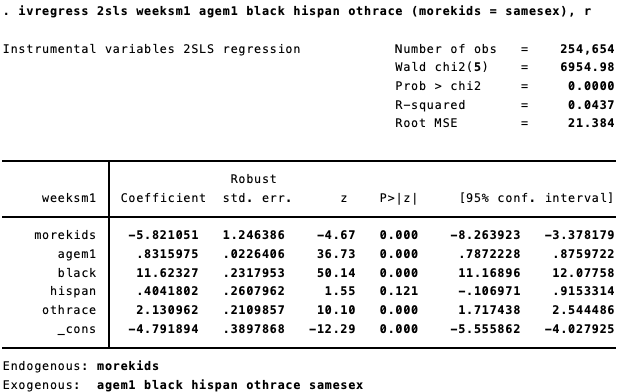
\includegraphics[width=0.8\linewidth]{pictures/res6-ivregress2SLS} \end{center}
\end{frame}

\begin{frame}[fragile]{(g) How large is the fertility effect on labor
supply?}
\protect\hypertarget{g-how-large-is-the-fertility-effect-on-labor-supply}{}
\begin{itemize}
\item
  Estimation result \[
  \hat{\beta}_1^{TSLS} \approx -5.82, \quad \text{robust s.e} \approx 1.25 
  \]
\item
  The results do not change in an important way. The reason is that
  \texttt{samesex} is unrelated to \texttt{agem1}, \texttt{black},
  \texttt{hispan}, \texttt{othrace}. Thus its covariance with these
  variables is zero, and thus \texttt{samesex} is likely to be
  uncorrelated with the error term, even when the latter includes those
  variables.
\end{itemize}
\end{frame}

\begin{frame}[fragile]{(g) Check Instrument Relevance}
\protect\hypertarget{g-check-instrument-relevance}{}
\small

\begin{Shaded}
\begin{Highlighting}[]
\NormalTok{* ivregress 2sls yvar wvar1 wvar2 wvark (xvar = IV), }\FunctionTok{r}
\NormalTok{* }\KeywordTok{estat}\NormalTok{ firststage}
\end{Highlighting}
\end{Shaded}

\begin{center}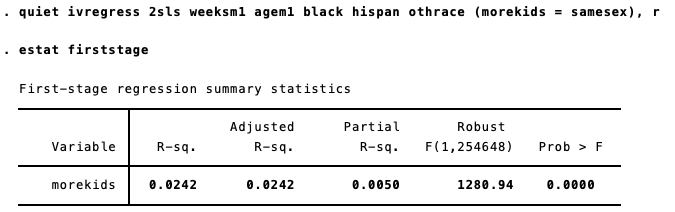
\includegraphics[width=0.9\linewidth]{pictures/res7-estatFirstStage2SLS} \end{center}

\(\Rightarrow\) The instrument \texttt{samesex} remains relevant. The
reason is that the addition of the new variables does not affect the
strength of the relationship between \texttt{morekids} and
\texttt{samesex}.
\end{frame}

\begin{frame}[fragile]{(g) Test endogeneity of regressor \(X:morekids\)}
\protect\hypertarget{qa-endog}{}
\small

\begin{Shaded}
\begin{Highlighting}[]
\NormalTok{* ivregress 2sls yvar wvar1 wvar2 wvark (xvar = IV), }\FunctionTok{r}
\NormalTok{* }\KeywordTok{estat}\NormalTok{ endog}
\end{Highlighting}
\end{Shaded}

\begin{center}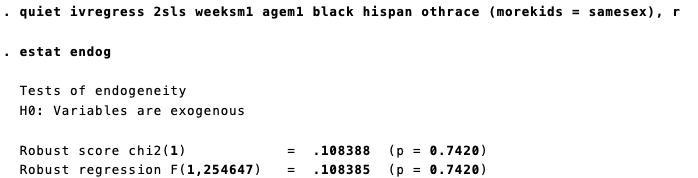
\includegraphics[width=0.9\linewidth]{pictures/res8-estatEndog2SLS} \end{center}

\(\Rightarrow\) The endogeneity test gives the same result as without
the additional regressors. However, we should still be very skeptical
about the possibility of \texttt{morekids} being exogenous.
\footnotesize\protect\hyperlink{review-endog}{(\textgreater\textgreater review)}
\normalsize
\end{frame}

\begin{frame}{Table of Results}
\protect\hypertarget{table-of-results}{}
\small

\begin{table}[]
\begin{tabular}{@{}|l|ccc|@{}}
\toprule
\multirow{2}{*}{\textbf{Regressor}} & \multicolumn{3}{c|}{\textbf{Estimation method}}                                        \\ \cmidrule(l){2-4} 
                                    & \multicolumn{1}{c|}{\textbf{OLS}} & \multicolumn{1}{c|}{\textbf{TSLS}} & \textbf{TSLS} \\ \midrule
\textit{morekids} &
  \multicolumn{1}{c|}{\begin{tabular}[c]{@{}c@{}}\color{red}{-5.39}\\ (0.09)\\ {[}-5.56, -5.22{]}\end{tabular}} &
  \multicolumn{1}{c|}{\begin{tabular}[c]{@{}c@{}}\color{red}{-6.31}\\ (1.27)\\ {[}-8.81, -3.81{]}\end{tabular}} &
  \begin{tabular}[c]{@{}c@{}}\color{red}{-5.82}\\ (1.25)\\ {[}-8.26, -3.38{]}\end{tabular} \\ \midrule
\textit{Additional regressors} &
  \multicolumn{1}{l|}{\textit{Intercept}} &
  \multicolumn{1}{l|}{\textit{Intercept}} &
  \multicolumn{1}{l|}{\textit{\begin{tabular}[c]{@{}l@{}}Intercept, agem1,\\ black, hispan, othrace\end{tabular}}} \\ \midrule
First Stage F-Statistic             & \multicolumn{1}{l|}{}             & \multicolumn{1}{c|}{1238.2}        & 1280.9        \\ \bottomrule
\end{tabular}
\end{table}

\footnotesize Notes: Standard errors shown in parentheses and 95\%
confidence intervals are shown in brackets.
\end{frame}

\hypertarget{brief-review}{%
\section{BRIEF REVIEW}\label{brief-review}}

\begin{frame}{Causal Graph (I)}
\protect\hypertarget{LGCG}{}
\begin{block}{Linear regression}
\protect\hypertarget{linear-regression-1}{}
\begin{center}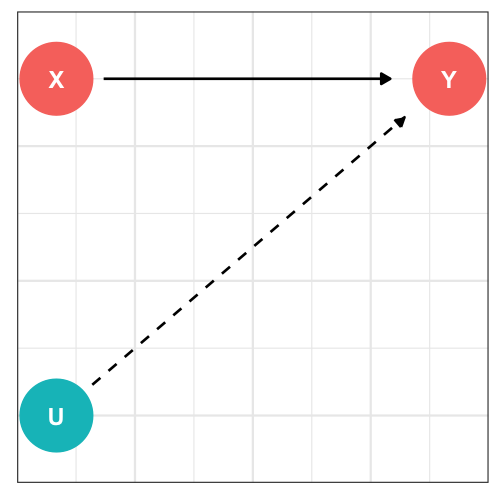
\includegraphics[width=0.4\linewidth,height=0.54\textheight]{pictures/LGsetting1} 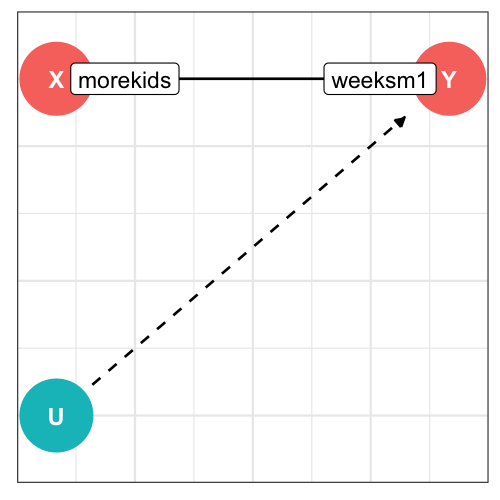
\includegraphics[width=0.4\linewidth,height=0.54\textheight]{pictures/LGsetting2} \end{center}

\[
E(u_i \mid X_i) = 0
\] \footnotesize\protect\hyperlink{LGQ}{(\textgreater\textgreater back)}
\normalsize
\end{block}
\end{frame}

\begin{frame}{Causal Graph (II)}
\protect\hypertarget{IVCG}{}
\begin{block}{IV regression with a single regressor and a single
instrument}
\protect\hypertarget{iv-regression-with-a-single-regressor-and-a-single-instrument-1}{}
\begin{center}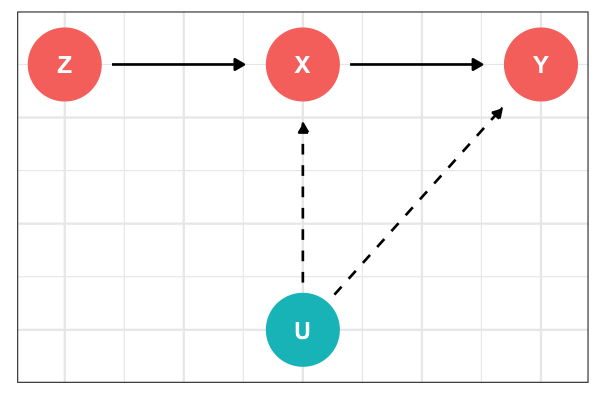
\includegraphics[width=0.48\linewidth,height=0.4\textheight]{pictures/IVsetting1} 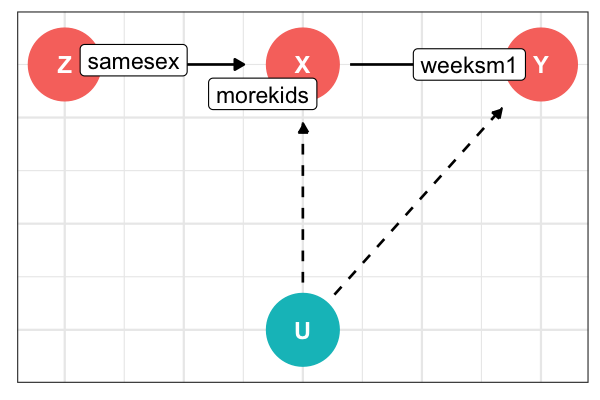
\includegraphics[width=0.48\linewidth,height=0.4\textheight]{pictures/IVsetting2} \end{center}

\[
\underset{\color{gray}{relevance}}{\text{corr}(Z_i, X_i)} \neq 0 \text{ and } \underset{\color{gray}{exogeneity}}{\text{corr}(Z_i, u_i)}  = 0
\] \footnotesize\protect\hyperlink{IVQ}{(\textgreater\textgreater back)}
\normalsize
\end{block}
\end{frame}

\begin{frame}{Causal Graph (III)}
\protect\hypertarget{IVCCG}{}
\begin{block}{IV regression with additional control variables}
\protect\hypertarget{iv-regression-with-additional-control-variables-1}{}
\begin{center}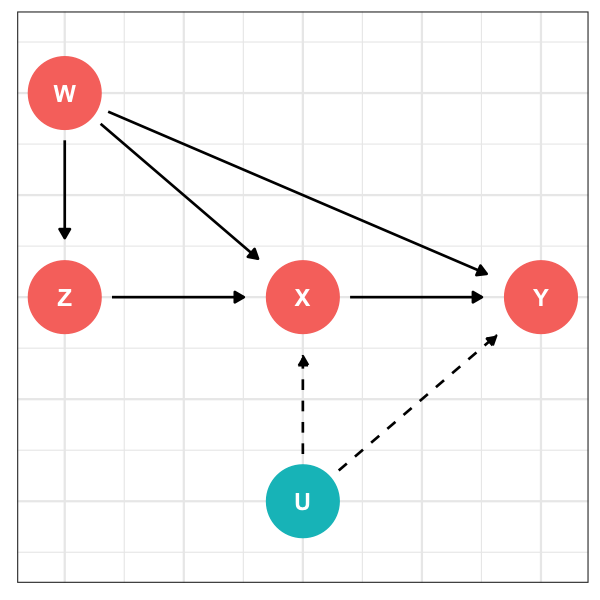
\includegraphics[width=0.48\linewidth,height=0.58\textheight]{pictures/IVCsetting1} 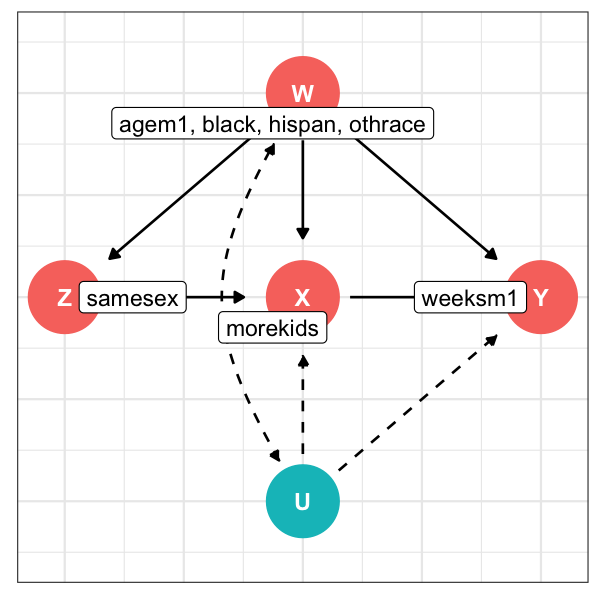
\includegraphics[width=0.48\linewidth,height=0.58\textheight]{pictures/IVCsetting2} \end{center}

\[
E(u_i \mid Z_i, W_i) = E(u_i \mid W_i) = 0
\]
\footnotesize\protect\hyperlink{IVCQ}{(\textgreater\textgreater back)}
\normalsize
\end{block}
\end{frame}

\begin{frame}{Omitted Variable Bias}
\protect\hypertarget{OVB}{}
\begin{itemize}
\tightlist
\item
  If there is another factor \(F\) that is a determinant of \(Y\) and
  correlated with \(X\) which makes \(X\) and \(Y\) be associated,
  ignoring \(F\) will cause omitted variable bias
\end{itemize}

\[
    plim\hat{\beta_1} = \beta_1 + \beta_2\frac{Cov(X,F)}{Var(X)}
\]

\begin{itemize}
\tightlist
\item
  \(\hat{\beta_1}\) is biased \textcolor{red}{upward} \hspace{3mm}
  \(\Leftrightarrow\) \textcolor{red}{$plim\hat{\beta_1} > \beta_1$}
\item
  \(\hat{\beta_1}\) is biased \textcolor{green}{downward}
  \(\Leftrightarrow\) \textcolor{green}{$plim\hat{\beta_1} < \beta_1$}
\end{itemize}

\vspace{3mm}

\begin{center}
\setlength{\tabcolsep}{3pt}
\begin{tabular}{|c|c|c|}
\hline
& $Cov(X,F) > 0$ & $Cov(X,F) < 0$
\\
\hline
$\beta_2 > 0$ & \textcolor{red}{$plim\hat{\beta_1} > \beta_1$}  & \textcolor{green}{$plim\hat{\beta_1} < \beta_1$} \\
 \hline 
$\beta_2 < 0$ & \textcolor{green}{$plim\hat{\beta_1} < \beta_1$} & \textcolor{red}{$plim\hat{\beta_1} > \beta_1$}
\\ \hline
\end{tabular}
\end{center}

\footnotesize \protect\hyperlink{LRissue}{(\textgreater\textgreater backB)}
\normalsize
\end{frame}

\begin{frame}{Testing for regressor endogeneity (I)}
\protect\hypertarget{review-endog}{}
\begin{enumerate}
\tightlist
\item
  Hausman test
\end{enumerate}

\begin{itemize}
\item
  If there is little difference between OLS and IV estimators, then
  there is no need to instrument, and we conclude that the regressor was
  exogenous.
\item
  If instead there is considerable difference, then we needed to
  instrument and the regressor is endogenous.
\item
  Idea: Compares just the coefficients of the endogenous variables, with
  the use of the Hausman test statistic \[
  T_H = \frac{(\hat\beta_{IV} - \hat\beta_{OLS})^2}{\hat V (\hat\beta_{IV} - \hat\beta_{OLS})} \sim \chi^2(1)
  \]
\item
  It relies on a very strong assumption that model errors are
  independent and homoskedastic.
\end{itemize}
\end{frame}

\begin{frame}{Testing for regressor endogeneity (II)}
\protect\hypertarget{testing-for-regressor-endogeneity-ii}{}
\begin{enumerate}
\setcounter{enumi}{1}
\tightlist
\item
  Durbin-Wu-Hausman (DWH) test
\end{enumerate}

\begin{itemize}
\item
  Idea: Use augmented regressors to produce a robust test statistic.
  Specifically, rewrite the structural equation with an additional
  variable \[
  Y_i = \beta X_i + \mathbf{W}_i\mathbf{\gamma} + \rho v_i + u_i
  \] Under Null hypothesis that \(D_i\) is exogenous,
  \(E(v_iu_i\mid D_i \mathbf{X}_i) = 0\).
\item
  Null hypothesis becomes: \[
  H_0: \rho = 0
  \]
\item
  Valid even in the case of heteroskedastic errors provided that we use
  robust variance estimates.
\end{itemize}

\footnotesize\protect\hyperlink{qa-endog}{(\textgreater\textgreater backG)}
\normalsize
\end{frame}

\hypertarget{stata-codes-results}{%
\section{STATA CODES \& RESULTS}\label{stata-codes-results}}

\begin{frame}[fragile]{}
\protect\hypertarget{res1-regOLS}{}
\small

\begin{Shaded}
\begin{Highlighting}[]
\NormalTok{* }\KeywordTok{regress}\NormalTok{ yvar xvar, }\FunctionTok{r}
\CommentTok{// add option r to report Hetroskedasticity{-}robust standard errors}
\end{Highlighting}
\end{Shaded}

\begin{center}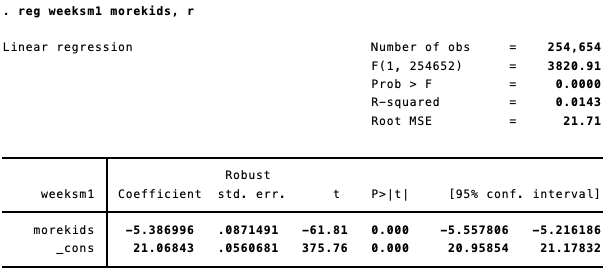
\includegraphics[width=1\linewidth]{pictures/res1-regOLS} \end{center}

\footnotesize \protect\hyperlink{q1-regOLS}{(\textgreater\textgreater backA)}
\normalsize
\end{frame}

\begin{frame}[fragile]{}
\protect\hypertarget{res2-regFirstStage}{}
\small

\begin{Shaded}
\begin{Highlighting}[]
\NormalTok{* }\KeywordTok{regress}\NormalTok{ xvar IV, }\FunctionTok{r}
\CommentTok{// add option r to report Hetroskedasticity{-}robust standard errors}
\end{Highlighting}
\end{Shaded}

\begin{center}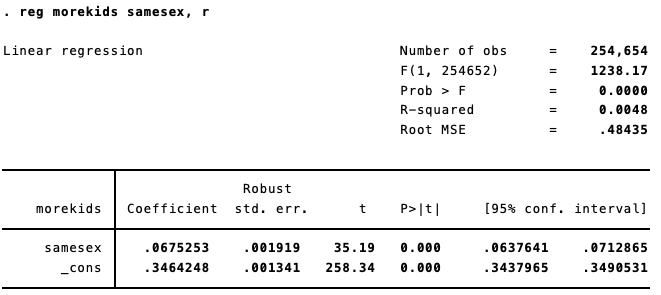
\includegraphics[width=1\linewidth]{pictures/res2-regFirstStage} \end{center}

\footnotesize \protect\hyperlink{q2-regFirstStage}{(\textgreater\textgreater backC)}
\normalsize
\footnotesize \protect\hyperlink{IVestatFirstStage}{(\textgreater\textgreater backF)}
\normalsize
\end{frame}

\begin{frame}[fragile]{}
\protect\hypertarget{section}{}
\small

\begin{Shaded}
\begin{Highlighting}[]
\NormalTok{* ivregress 2sls yvar (xvar = IV), }\FunctionTok{r}
\CommentTok{// report result of intrinsic interest with 2SLS estimate}
\end{Highlighting}
\end{Shaded}

\begin{center}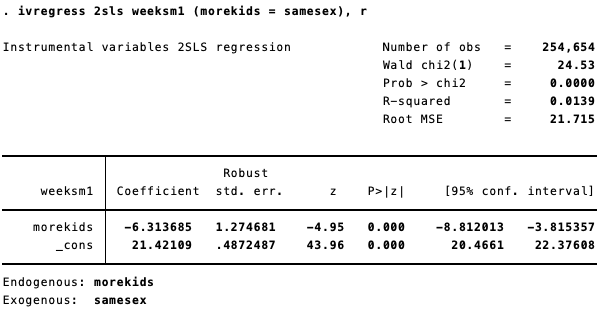
\includegraphics[width=1\linewidth]{pictures/res3-ivregress} \end{center}
\end{frame}

\begin{frame}[fragile]{}
\protect\hypertarget{section-1}{}
\small

\begin{Shaded}
\begin{Highlighting}[]
\NormalTok{* ivregress 2sls yvar (xvar = IV), }\FunctionTok{r}
\NormalTok{* }\KeywordTok{estat}\NormalTok{ firststage}
\CommentTok{// report first{-}stage regression statistics}
\end{Highlighting}
\end{Shaded}

\begin{center}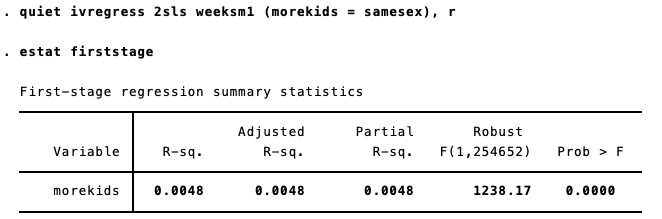
\includegraphics[width=1\linewidth]{pictures/res4-estatFirstStage} \end{center}
\end{frame}

\begin{frame}[fragile]{}
\protect\hypertarget{section-2}{}
\small

\begin{Shaded}
\begin{Highlighting}[]
\NormalTok{* ivregress 2sls yvar (xvar = IV), }\FunctionTok{r}
\NormalTok{* }\KeywordTok{estat}\NormalTok{ endog}
\CommentTok{// perform tests of the endogeneity of xvar}
\end{Highlighting}
\end{Shaded}

\begin{center}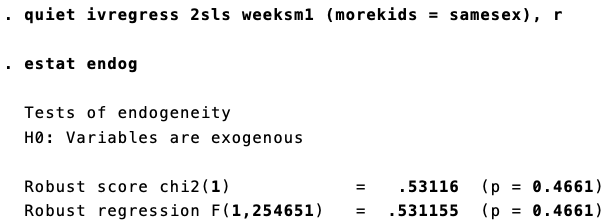
\includegraphics[width=1\linewidth]{pictures/res5-estatEndog} \end{center}
\end{frame}

\begin{frame}[fragile]{}
\protect\hypertarget{section-3}{}
\small

\begin{Shaded}
\begin{Highlighting}[]
\NormalTok{* ivregress 2sls yvar wvar1 wvar2 wvark (xvar = IV), }\FunctionTok{r}
\CommentTok{// report result of intrinsic interest with 2SLS estimate}
\end{Highlighting}
\end{Shaded}

\begin{center}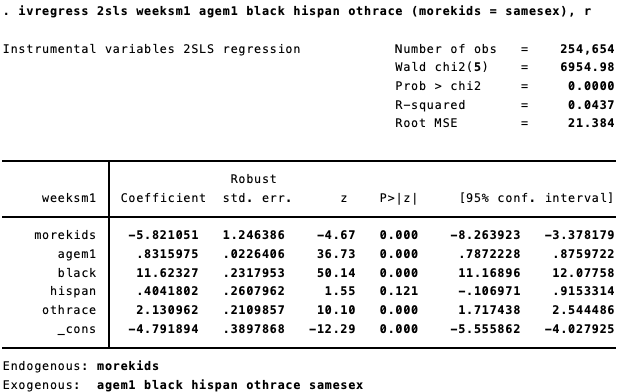
\includegraphics[width=1\linewidth]{pictures/res6-ivregress2SLS} \end{center}
\end{frame}

\begin{frame}[fragile]{}
\protect\hypertarget{section-4}{}
\small

\begin{Shaded}
\begin{Highlighting}[]
\NormalTok{* ivregress 2sls yvar wvar1 wvar2 wvark (xvar = IV), }\FunctionTok{r}
\NormalTok{* }\KeywordTok{estat}\NormalTok{ firststage}
\CommentTok{// report first{-}stage regression statistics}
\end{Highlighting}
\end{Shaded}

\begin{center}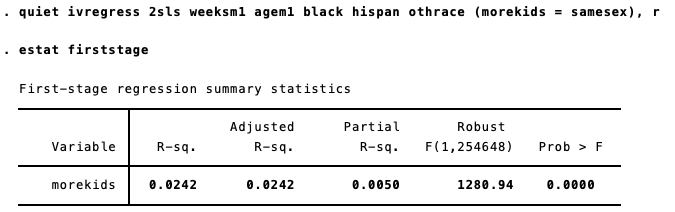
\includegraphics[width=1\linewidth]{pictures/res7-estatFirstStage2SLS} \end{center}
\end{frame}

\begin{frame}[fragile]{}
\protect\hypertarget{section-5}{}
\small

\begin{Shaded}
\begin{Highlighting}[]
\NormalTok{* ivregress 2sls yvar wvar1 wvar2 wvark (xvar = IV), }\FunctionTok{r}
\NormalTok{* }\KeywordTok{estat}\NormalTok{ endog}
\CommentTok{// perform tests of the endogeneity of xvar}
\end{Highlighting}
\end{Shaded}

\begin{center}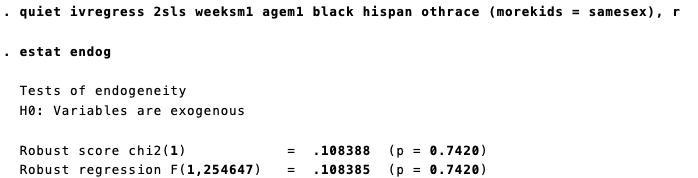
\includegraphics[width=1\linewidth]{pictures/res8-estatEndog2SLS} \end{center}
\end{frame}

\end{document}
